\begin{name}
	{\tenchude}{\tendethi}{LỚP TOÁN THẦY PHÁT}{\thoigian}
\end{name}
\setcounter{ex}{0}

\Opensolutionfile{ans}[ans/ans-2-TT-20-SoGDDT-YenBai-23]
\begin{ex}%[Đề thi thử Sở Yên Bái - 22 - 23]%[Dự án 12EX-6-2023]%[Nhật Thiện]%[2D1Y5-1]
	\immini{Đồ thị của hàm số nào dưới đây có dạng như hình bên?
		\choice
		{\True $y=x^3-6x^2+9x-2$}
		{$y=-x^4+3x^2-2$}
		{$y=x^4-3x^2-2$}
		{$y=-x^3+6x^2-9x-2$}}{
		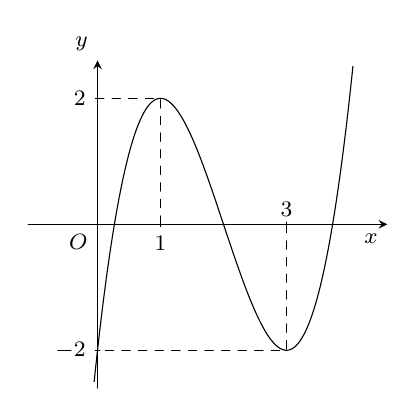
\begin{tikzpicture}[scale=1, font=\footnotesize, line join=round, line cap=round, >=stealth]
			\begin{scope}[scale=.8]
				\draw[->] (-1.1,0)--(4.6,0) node[below left] {$x$};
				\draw[->] (0,-2.6)--(0,2.6) node[above left] {$y$};
				\draw (0,0) node [below left] {$O$};
				\draw[dashed,thin](1,0)--(1,2)--(0,2);
				\draw[dashed,thin](3,0)--(3,-2)--(0,-2);
				\begin{scope}
					\clip (-1,-2.5) rectangle (4.5,2.5);
					\draw[samples=200,domain=-1:4.5,smooth,variable=\x] plot (\x,{1*((\x)^3)+-6*((\x)^2)+9*(\x)+-2});
				\end{scope}
				\draw (1,1pt)--(1,-1pt) node[below]{$1$} (3,1pt)--(3,-1pt) node[above]{$3$};
				\foreach \y in {2,-2} \draw (1pt,\y)--(-1pt,\y) node[left]{$\y$};
			\end{scope}
		\end{tikzpicture}
	}
	\loigiai{
		Dựa vào hình vẽ, ta thấy
		\begin{itemize}
			\item Hàm số có dạng hàm số bậc ba $y=ax^3+bx^2+cx+d$.
			\item $\lim\limits_{x\to +\infty} y=+\infty$ suy ra $a>0$.
			\item Đồ thị hàm số có hai điểm cực trị $(1,2)$ và $(3,-2)$.
		\end{itemize}
		Vậy hình vẽ là đồ thị của hàm số $y=x^3-6x^2+9x-2$.
	}
\end{ex}
\begin{ex}%[Đề thi thử Sở Yên Bái - 22 - 23]%[Dự án 12EX-6-2023]%[Nhật Thiện]%[2D1Y1-2]
	Cho hàm số $y=f(x)$ có bảng biến thiên như sau
	\begin{center}
		
\begin{tikzpicture}[scale=1, font=\footnotesize, line join=round, line cap=round, >=stealth]
			\tkzTabInit[nocadre=false,lgt=1.2,espcl=2.5,deltacl=0.6]
			{$x$ /0.6,$y’$ /0.6,$y$ /2}
			{$-\infty$,$-1$,$1$,$+\infty$}
			\tkzTabLine{,+,0,-,0,+,}
			\tkzTabVar{-/$-\infty$,+/$4$,-/$-1$,+/$+\infty$}
		\end{tikzpicture}
	\end{center}
	Hàm số đã cho nghịch biến trên khoảng
	\choice
	{$(-1;4)$}
	{$(-\infty;0)$}
	{$(-1;+\infty)$}
	{\True $(-1;1)$}
	\loigiai{
		Dựa vào bảng biến thiên, hàm số đã cho nghịch biến trên khoảng $(-1;1)$.
	}
\end{ex}
\begin{ex}%[Đề thi thử Sở Yên Bái - 22 - 23]%[Dự án 12EX-6-2023]%[Nhật Thiện]%[2H3Y3-1]
	Trong không gian $Oxyz$, đường thẳng $d\colon \dfrac{x-2}{-1}=\dfrac{y-1}{2}=\dfrac{z-3}{1}$ có một véc-tơ chỉ phương là
	\choice
	{$\vec{u}_1=(-1;2;3)$}
	{$\vec{u}_3=(2;1;3)$}
	{$\vec{u}_2=(2;1;1)$}
	{\True $\vec{u}_4=(-1;2;1)$}
	\loigiai{
		Đường thẳng $d\colon \dfrac{x-2}{-1}=\dfrac{y-1}{2}=\dfrac{z-3}{1}$ có một véc-tơ chỉ phương là $\vec{a}=(-1;2;1)=\vec{u}_4$.
	}
\end{ex}
\begin{ex}%[Đề thi thử Sở Yên Bái - 22 - 23]%[Dự án 12EX-6-2023]%[Nhật Thiện]%[2H3Y1-1]
	Trong không gian $Oxyz$, cho điểm $M(0;2023;-5)$. Mệnh đề nào dưới đây đúng?
	\choice
	{\True $M\in (Oyz)$}
	{$M\in (Oxz)$}
	{$M\in Oy$}
	{$M\in (Oxy)$}
	\loigiai{
		Xét thấy điểm $M(0;2023;-5)\in (Oyz)$.
	}
\end{ex}
\begin{ex}%[Đề thi thử Sở Yên Bái - 22 - 23]%[Dự án 12EX-6-2023]%[Nhật Thiện]%[2H3Y1-1]
	Trong không gian $Oxyz$, cho điểm $M(2;-1;4)$. Tọa độ điểm $N$ đối xứng với điểm $M$ qua mặt phẳng $(Oxz)$ là
	\choice
	{$(-2;1;-4)$}
	{$(2;0;4)$}
	{\True $(2;1;4)$}
	{$(0;-1;0)$}
	\loigiai{
		Tọa độ điểm $N$ đối xứng với điểm $M(2;-1;4)$ qua mặt phẳng $(Oxz)$ có tọa độ là $(2;1;4)$.
	}
\end{ex}
\begin{ex}%[Đề thi thử Sở Yên Bái - 22 - 23]%[Dự án 12EX-6-2023]%[Nhật Thiện]%[2D4Y1-1]
	Mô-đun của số phức $z=4+i$ bằng
	\choice
	{\True $\sqrt{17}$}
	{$17$}
	{$4$}
	{$\sqrt{5}$}
	\loigiai{
		Ta có $|z|=\sqrt{4^2+1^2}=\sqrt{17}$.
	}
\end{ex}
\begin{ex}%[Đề thi thử Sở Yên Bái - 22 - 23]%[Dự án 12EX-6-2023]%[Nhật Thiện]%[2D1Y2-2]
	\immini{Cho hàm số bậc ba $y=f(x)$ có đồ thị như hình bên. Giá trị cực đại của hàm số đã cho là
		\choice
		{$-1$}
		{\True $2$}
		{$1$}
		{$-2$}}{
		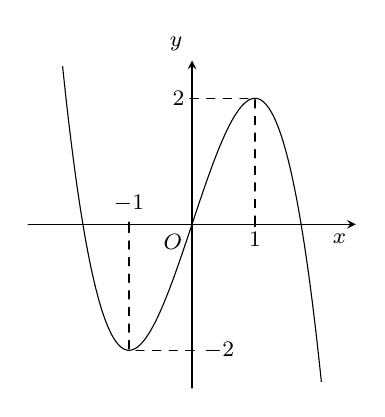
\begin{tikzpicture}[scale=1, font=\footnotesize, line join=round, line cap=round, >=stealth]
			\begin{scope}[scale=.8]
				\draw[->] (-2.6,0)--(2.6,0) node[below left] {$x$};
				\draw[->] (0,-2.6)--(0,2.6) node[above left] {$y$};
				\draw (0,0) node [below left] {$O$};
				\draw[dashed,thin](-1,0)--(-1,-2)--(0,-2);
				\draw[dashed,thin](1,0)--(1,2)--(0,2);
				\begin{scope}
					\clip (-2.5,-2.5) rectangle (2.5,2.5);
					\draw[samples=200,domain=-2.5:2.5,smooth,variable=\x] plot (\x,{-1*((\x)^3)+0*((\x)^2)+3*(\x)+0});
				\end{scope}
				\draw (1,-1pt)--(1,1pt) node[below]{$1$} (-1,-1pt)--(-1,1pt) node[above]{$-1$} (-1pt,-2)--(1pt,-2) node[right]{$-2$} (-1pt,2)--(1pt,2)node[left]{$2$};
			\end{scope}
		\end{tikzpicture}
	}
	\loigiai{
		Dựa vào đồ thị, giá trị cực đại của hàm số đã cho là $y=2$.
	}
\end{ex}
%C:\Users\dnthi\OneDrive\THAM_GIA_TREN_MANG\12EX-2019\2-TT-20-SoGDDT-YenBai-23.tex
\begin{ex}%[Đề thi thử Sở Yên Bái - 22 - 23]%[Dự án 12EX-6-2023]%[Nhật Thiện]%[2D3Y1-1]
	Cho hàm số $f(x)=\mathrm{e}^x+\dfrac{1}{\cos^2x}$. Khẳng định nào đúng?
	\choice
	{$\displaystyle\int f(x) \mathrm{\,d}x=\mathrm{e}^x-\dfrac{1}{\cos x}+C$}
	{\True $\displaystyle\int f(x) \mathrm{\,d}x=\mathrm{e}^x+\tan x+C$}
	{$\displaystyle\int f(x) \mathrm{\,d}x=\mathrm{e}^x-\tan x+C$}
	{$\displaystyle\int f(x) \mathrm{\,d}x=\mathrm{e}^x+\dfrac{1}{\cos x}+C$}
	\loigiai{
		Ta có $\displaystyle\int f(x) \mathrm{\,d}x=\displaystyle\int \left(\mathrm{e}^x+\dfrac{1}{\cos^2x} \right) \mathrm{\,d}x= \mathrm{e}^x+\tan x+C$.
	}
\end{ex}
\begin{ex}%[Đề thi thử Sở Yên Bái - 22 - 23]%[Dự án 12EX-6-2023]%[Nhật Thiện]%[2H3Y2-2]
	Trong không gian $Oxyz$, mặt phẳng $(P)\colon 3x-z+2=0$ có một véc-tơ pháp tuyến là
	\choice
	{$\vec{n}_2=(3;-1;0)$}
	{\True $\vec{n}_3=(3;0;-1)$}
	{$\vec{n}_1=(3;-1;2)$}
	{$\vec{n}_4=(-1;0;-1)$}
	\loigiai{
		Mặt phẳng $(P)\colon 3x-z+2=0$ có một véc-tơ pháp tuyến là $\vec{n}=(3;0;-1)=\vec{n}_3$.
	}
\end{ex}
\begin{ex}%[Đề thi thử Sở Yên Bái - 22 - 23]%[Dự án 12EX-6-2023]%[Nhật Thiện]%[2D1Y4-1]
	Tiệm cận ngang của đồ thị hàm số $y=\dfrac{x+1}{2x-4}$ là đường thẳng có phương trình là
	\choice
	{$x=2$}
	{$x=-1$}
	{$y=-\dfrac{1}{4}$}
	{\True $y=\dfrac{1}{2}$}
	\loigiai{
		Xét hàm số $y=\dfrac{x+1}{2x-4}$, tập xác định $\mathscr{D}=\mathbb{R}\setminus \{2\}$.\\
		Ta có $\lim\limits_{x\to +\infty} y=\dfrac{1}{2}$ và $\lim\limits_{x\to -\infty} y=\dfrac{1}{2}$.\\
		Vậy $y=\dfrac{1}{2}$ là tiệm cận ngang của đồ thị hàm số đã cho.
	}
\end{ex}
\begin{ex}%[Đề thi thử Sở Yên Bái - 22 - 23]%[Dự án 12EX-6-2023]%[Nhật Thiện]%[1D2Y2-1]
	Có bao nhiêu cách sắp xếp $7$ học sinh thành một hàng dọc?
	\choice
	{$7^7$}
	{$6!$}
	{$7$}
	{\True $7!$}
	\loigiai{
		Xếp $7$ học sinh thành một hàng dọc có $7!$ cách.
	}
\end{ex}
\begin{ex}%[Đề thi thử Sở Yên Bái - 22 - 23]%[Dự án 12EX-6-2023]%[Nhật Thiện]%[2H1Y3-2]
	Cho khối lăng trụ có diện tích đáy $B=3a^2$ và chiều cao $h=a$. Thể tích của khối lăng trụ đã cho bằng
	\choice
	{$\dfrac{3}{2}a^3$}
	{$\dfrac{1}{2}a^3$}
	{$a^3$}
	{\True $3a^3$}
	\loigiai{
		Thế tích của khối lăng trụ có diện tích đáy $B=3a^2$ và chiều cao $h=a$ là
		$$V=B\cdot h=3a^2\cdot a=3a^3.$$
	}
\end{ex}
\begin{ex}%[Đề thi thử Sở Yên Bái - 22 - 23]%[Dự án 12EX-6-2023]%[Nhật Thiện]%[2H1Y3-2]
	Cho hình chóp $S.ABCD$ có đáy $ABCD$ là hình vuông cạnh $a$, $SA\perp (ABCD)$, $SA=a\sqrt{2}$. Thể tích $V$ của khối chóp $S.ABCD$ bằng
	\choice
	{\True $V=\dfrac{a^3\sqrt{2}}{3}$}
	{$V=\dfrac{a^3\sqrt{2}}{6}$}
	{$V=\dfrac{a^3\sqrt{2}}{4}$}
	{$V=a^3\sqrt{2}$}
\loigiai{
Thể tích $V$ của khối chóp $S.ABCD$ bằng
$$V=\dfrac{1}{3}\cdot S_{ABCD}\cdot SA=\dfrac{1}{3}\cdot AB^2\cdot SA=\dfrac{1}{3}\cdot a^2\cdot a\sqrt{2}=\dfrac{a^3\sqrt{2}}{3}.$$
}
\end{ex}
\begin{ex}%[Đề thi thử Sở Yên Bái - 22 - 23]%[Dự án 12EX-6-2023]%[Nhật Thiện]%[2H3Y1-3]
	Trong không gian $Oxyz$, tọa độ tâm của mặt cầu $(S)\colon x^2+y^2+2x-8z-1=0$ là
	\choice
	{\True $I(-1;0;4)$}
	{$I(1;-4;0)$}
	{$I(2;-8;0)$}
	{$I(-2;8;0)$}
	\loigiai{
		Mặt cầu $(S)\colon x^2+y^2+2x-8z-1=0$ có $a=-1$, $b=0$, $c=4$, $d=-1$.\\
		Vậy tâm mặt cầu $(S)$ là $I(-1;0;4)$.
	}
\end{ex}
\begin{ex}%[Đề thi thử Sở Yên Bái - 22 - 23]%[Dự án 12EX-6-2023]%[Nhật Thiện]%[2D4B2-2]
	Cho hai số phức $z_1=1+i$ và $z_2=3-2i$. Phần ảo của số phức $2z_1+\bar{z_2}$ bằng
	\choice
	{$-2$}
	{\True $4$}
	{$0$}
	{$-4$}
	\loigiai{
		Xét số phức $w=2z_1+\bar{z_2}=2(1+i)+(3+2i)=5+4i$.\\
		Phần ảo của số phức $w$ bằng $4$.
	}
\end{ex}
\begin{ex}%[Đề thi thử Sở Yên Bái - 22 - 23]%[Dự án 12EX-6-2023]%[Nhật Thiện]%[2D2B5-1]
	Tập nghiệm của phương trình $2023^{x^2-5x+6}=1$ là
	\choice
	{$\{0;2023\}$}
	{\True $\{2;3\}$}
	{$\{-3;2\}$}
	{$\{-2;3\}$}
	\loigiai{
		Ta có $2023^{x^2-5x+6}=1\Leftrightarrow x^2-5x+6=\log_{2023}1=0\Leftrightarrow \hoac{&x=2\\&x=3.}$\\
		Vậy tập nghiệm của phương trình là $\{2;3\}$.
	}
\end{ex}
\begin{ex}%[Đề thi thử Sở Yên Bái - 22 - 23]%[Dự án 12EX-6-2023]%[Nhật Thiện]%[2D2B3-2]
	Với $a$ là số thực dương tùy ý, $\log_3\sqrt{a}$ bằng
	\choice
	{$2+\log_3a$}
	{\True $\dfrac{1}{2}\log_3a$}
	{$\dfrac{1}{2}+\log_3a$}
	{$2\log_3a$}
\loigiai{
Với $a$ là số thực dương tùy ý, ta có
$$\log_3\sqrt{a}=\log_3 a^{\frac{1}{2}}=\dfrac{1}{2}\log_3a.$$
}
\end{ex}

\begin{ex}%[Đề thi thử Sở Yên Bái - 22 - 23]%[Dự án 12EX-6-2023]%[Nhật Thiện]%[2D3B2-1]
	Nếu $\displaystyle\int\limits_0^3 f(x) \mathrm{\,d}x=1$ và $\displaystyle\int\limits_3^5 f(x) \mathrm{\,d}x=-5$ thì $\displaystyle\int\limits_0^5 f(x) \mathrm{\,d}x$ bằng
	\choice
	{$6$}
	{$-5$}
	{\True $-4$}
	{$-6$}
\loigiai{
Ta có $\displaystyle\int\limits_0^5 f(x) \mathrm{\,d}x=\displaystyle\int\limits_0^3 f(x) \mathrm{\,d}x+\displaystyle\int\limits_3^5 f(x) \mathrm{\,d}x=1+(-5)=-4$.
}
\end{ex}
\begin{ex}%[Đề thi thử Sở Yên Bái - 22 - 23]%[Dự án 12EX-6-2023]%[Nhật Thiện]%[2D2B3-2]
	Cho các số thực dương $a$, $b$ thỏa mãn $\ln a=x$, $\ln b=y$. Tính $P=\ln \left(a^3b^2\right)$.
	\choice
	{$P=x^2y^3$}
	{\True $P=3x+2y$}
	{$P=6xy$}
	{$P=x^2+y^2$}
	\loigiai{
		Với $a$, $b$ là các số dương, ta có 
		$$P=\ln \left(a^3 b^2\right)=\ln \left(a^3\right)+\ln \left(b^2\right)= 3\ln a+2\ln b= 3x+2y.$$
	}
\end{ex}
\begin{ex}%[Đề thi thử Sở Yên Bái - 22 - 23]%[Dự án 12EX-6-2023]%[Nhật Thiện]%[2D2B4-2]
	Trên khoảng $(0;+\infty)$, đạo hàm của hàm số $y=\ln 2023x$ là
	\choice
	{\True $y'=\dfrac{1}{x}$}
	{$y'=\dfrac{1}{2023x}$}
	{$y'=-\dfrac{2023}{x}$}
	{$y'=\dfrac{2023}{x}$}
	\loigiai{
		Xét trên khoảng $(0;+\infty)$, với $y=\ln 2023x$, ta có 
		$$y'=\dfrac{2023}{2023x}=\dfrac{1}{x}.$$
	}
\end{ex}
\begin{ex}%[Đề thi thử Sở Yên Bái - 22 - 23]%[Dự án 12EX-6-2023]%[Nhật Thiện]%[1D3B3-3]
	Cho cấp số cộng $(u_n)$ với $u_{10}=25$ và công sai $d=3$. Số hạng $u_1$ của cấp số cộng đã  cho bằng
	\choice
	{$u_1=2$}
	{$u_1=-3$}
	{\True $u_1=-2$}
	{$u_1=3$}
	\loigiai{
		Xét cấp số cộng $(u_n)$, ta có
		$$u_{10}=u_1+9d\Rightarrow u_1=u_{10}-9d=25-9\cdot 3=-2.$$
	}
\end{ex}

\begin{ex}%[Đề thi thử Sở Yên Bái - 22 - 23]%[Dự án 12EX-6-2023]%[Nhật Thiện]%[2H2B1-1]
	Cho hình nón có đường kính đáy $2r$ và độ dài đường cao $h$. Thể tích của khối nón đã cho bằng
	\choice
	{\True $\dfrac{1}{3}\pi r^2 h$}
	{$\pi r^2 h$}
	{$\dfrac{4}{3}\pi r^2 h$}
	{$\dfrac{2}{3}\pi r h^2$}
	\loigiai{
		Hình nón có bán kính đáy $r$ và độ dài đường cao $h$. Khi đó thể tích của khối nón bằng
		$V=\dfrac{1}{3} \pi r^2 h$.
	}
\end{ex}

\begin{ex}%[Đề thi thử Sở Yên Bái - 22 - 23]%[Dự án 12EX-6-2023]%[Nhật Thiện]%[2D1B2-1]
	Cho hàm số $f(x)$ có đạo hàm $f'(x)=x^2(x-1)(x+2)^3$, $\forall x\in \mathbb{R}$. Số điểm cực trị của hàm số đã cho là
	\choice
	{$1$}
	{$5$}
	{$3$}
	{\True $2$}
	\loigiai{
		Xét $f'(x)=0\Leftrightarrow \hoac{&x=0\\&x=1\\&x=-2.}$\\
		Ta có bảng biến thiên của hàm số $f(x)$ như sau
		\begin{center}
			
\begin{tikzpicture}[scale=1, font=\footnotesize, line join=round, line cap=round, >=stealth]
				\tkzTabInit[nocadre=false,lgt=1.2,espcl=2.5,deltacl=0.6]
				{$x$ /0.6,$f'(x)$ /0.6,$f(x)$ /2}
				{$-\infty$,$-2$,$0$,$1$,$+\infty$}
				\tkzTabLine{,+,0,-,0,-,0,+,}
				\tkzTabVar{-/,+/,R/,-/,+/}
			\end{tikzpicture}
		\end{center}
		Quan sát bảng biến thiên, hàm số $f(x)$ đã cho có $2$ điểm cực trị.
	}
\end{ex}
\begin{ex}%[Đề thi thử Sở Yên Bái - 22 - 23]%[Dự án 12EX-6-2023]%[Nhật Thiện]%[2D1B5-3]
	Cho hàm số $y=f(x)$ xác định, liên tục trên $\mathbb{R}$ và có bảng biến thiên như sau
	\begin{center}
		
\begin{tikzpicture}[scale=1, font=\footnotesize, line join=round, line cap=round, >=stealth]
\tkzTabInit[nocadre=false,lgt=1.2,espcl=2.5,deltacl=0.6]
{$x$ /0.6,$y’$ /0.6,$y$ /2}
{$-\infty$,$-1$,$0$,$1$,$+\infty$}
\tkzTabLine{,-,0,+,0,-,0,+,}
\tkzTabVar{+/$+\infty$,-/$-1$,+/$0$,-/$-1$,+/$+\infty$}
\end{tikzpicture}
	\end{center}
	Số nghiệm của phương trình $f(x)-2=0$ là
	\choice
	{\True $2$}
	{$0$}
	{$1$}
	{$3$}
\loigiai{
Ta có $f(x)-2=0\Leftrightarrow f(x)=2$.\\
Dựa vào bảng biến thiên, phương trình $f(x)=2$ có $2$ nghiệm phân biệt.
}
\end{ex}
\begin{ex}%[Đề thi thử Sở Yên Bái - 22 - 23]%[Dự án 12EX-6-2023]%[Nhật Thiện]%[2D4B4-1]
	Nghiệm phức có phần ảo dương của phương trình $z^2+2z+5=0$ là
	\choice
	{$1-2i$}
	{\True $-1+2i$}
	{$1+2i$}
	{$-1-2i$}
\loigiai{
Phương trình $z^2+2z+5=0\Leftrightarrow \hoac{&z=-1+2i\\&z=-1-2i.}$\\
Vậy nghiệm phức có phần ảo dương là $z=-1+2i$.
}
\end{ex}
\begin{ex}%[Đề thi thử Sở Yên Bái - 22 - 23]%[Dự án 12EX-6-2023]%[Nhật Thiện]%[2D3B3-1]
	Diện tích của hình phẳng giới hạn bởi đồ thị các hàm số $y=x^3-6x$ và $y=x^2$ bằng
	\choice
	{\True $\dfrac{253}{12}$}
	{$\dfrac{125}{12}$}
	{$\dfrac{63}{4}$}
	{$\dfrac{16}{3}$}
\loigiai{
	Phương trình hoành độ giao điểm của hai đồ thị hàm số $y=x^3-6x$ và $y=x^2$ là
	$$x^3-6x=x^2\Leftrightarrow x^3-x^2-6x=0\Leftrightarrow \hoac{&x=0\\&x=3\\&x=-2.}$$
	Diện tích hình phẳng giới hạn bởi hai đồ thị hàm số trên là
	\begin{eqnarray*}
		S&=& \displaystyle\int\limits_{-2}^0\left|(x^3-6x)-x^2\right| \mathrm{\,d}x+\displaystyle\int\limits_0^3 \left|(x^3-6x)-x^2\right| \mathrm{\,d}x\\
		&=& \displaystyle\int\limits_{-2}^0 \left|x^3-x^2-6x\right| \mathrm{\,d}x+\displaystyle\int\limits_0^3 \left|x^3-x^2-6x\right| \mathrm{\,d}x\\
		&=& \left|\displaystyle\int\limits_{-2}^0 (x^3-x^2-6x) \mathrm{\,d}x\right|+ \left|\displaystyle\int\limits_0^3 (x^3-x^2-6x) \mathrm{\,d}x\right|\\
		&=& \dfrac{16}{3}+\dfrac{63}{4}\\
		&=& \dfrac{253}{12}.
	\end{eqnarray*}

}
\end{ex}
\begin{ex}%[Đề thi thử Sở Yên Bái - 22 - 23]%[Dự án 12EX-6-2023]%[Nhật Thiện]%[2H3B3-2]
	Trong không gian $Oxyz$, phương trình đường thẳng đi qua hai điểm $P(1;1;-1)$ và $Q(2;3;2)$ là
	\choice
	{$\dfrac{x-1}{1}=\dfrac{y-2}{1}=\dfrac{z-3}{-1}$}
	{$\dfrac{x-1}{2}=\dfrac{y-1}{3}=\dfrac{z+1}{2}$}
	{$\dfrac{x+2}{1}=\dfrac{y+3}{2}=\dfrac{z+2}{3}$}
	{\True $\dfrac{x-1}{1}=\dfrac{y-1}{2}=\dfrac{z+1}{3}$}
\loigiai{
Đường thẳng đi qua hai điểm $P$ và $Q$ nhận $\vec{PQ}=(1;2;3)$ làm một véc-tơ chỉ phương.\\
Phương trình của đường thẳng $PQ$ là
$$\dfrac{x-1}{1}=\dfrac{y-1}{2}=\dfrac{z+1}{3}.$$
}
\end{ex}

\begin{ex}%[Đề thi thử Sở Yên Bái - 22 - 23]%[Dự án 12EX-6-2023]%[Nhật Thiện]%[2D2B6-1]
	Tập nghiệm của bất phương trình $\log_2(x-1)<1$ là
	\choice
	{$(-1;3)$}
	{$(-\infty;3)$}
	{$(3;+\infty)$}
	{\True $(1;3)$}
\loigiai{
Điều kiện bất phương trình $x-1>0\Leftrightarrow x>1$.\\
Bất phương trình $\log_2(x-1)<1\Leftrightarrow x-1<2^1\Leftrightarrow x<3$.\\
So sánh với điều kiện, tập nghiệm của bất phương trình trên là $S=(1;3)$.
}
\end{ex}
\begin{ex}%[Đề thi thử Sở Yên Bái - 22 - 23]%[Dự án 12EX-6-2023]%[Nhật Thiện]%[2H3B2-3]
	Trong không gian $Oxyz$, cho các điểm $A(1;1;2)$, $B(2;-2;1)$, $C(-2;0;1)$. Phương trình mặt phẳng đi qua $A$ và vuông góc với $BC$ là
	\choice
	{$y+2z-5=0$}
	{$2x-y+1=0$}
	{$-y+2z-3=0$}
	{\True $2x-y-1=0$}
\loigiai{
Mặt phẳng vuông góc với $BC$ nhận $\vec{BC}=(-4;2;0)=-2(2;-1;0)$ làm một véc-tơ pháp tuyến.\\
Mặt phẳng đi qua $A(1;1;2)$ có phương trình là
$$2(x-1)-1(y-1)+0(z-2)=0\Leftrightarrow 2x-y-1=0.$$
}
\end{ex}

\begin{ex}%[Đề thi thử Sở Yên Bái - 22 - 23]%[Dự án 12EX-6-2023]%[Nhật Thiện]%[2H2B2-1]
	Đường kính của khối cầu có thể tích $\dfrac{32\pi a^3}{3}$ bằng
	\choice
	{$a\sqrt{2}$}
	{$2a$}
	{\True $4a$}
	{$2a\sqrt{2}$}
\loigiai{
Thế tích khối cầu có bán kính $R$ là $V=\dfrac{4}{3}\pi R^3$.\\
Cho $V=\dfrac{32\pi a^3}{3}\Leftrightarrow \dfrac{4}{3}\pi R^3=\dfrac{32\pi a^3}{3} \Leftrightarrow R^3=8a^3\Leftrightarrow R=2a$.\\
Vậy đường kính của khối cầu bằng $2\cdot 2a=4a$.
}
\end{ex}
\begin{ex}%[Đề thi thử Sở Yên Bái - 22 - 23]%[Dự án 12EX-6-2023]%[Nhật Thiện]%[1H3B3-3]
	Cho hình chóp $S.ABC$ có đáy $ABC$ là tam giác đều cạnh bằng $a$, $SA\perp (ABC)$, $SA=a$. Tính góc giữa đường thẳng $SC$ và mặt phẳng $(ABC)$.
	\choice
	{$90^\circ$}
	{$60^\circ$}
	{\True $45^\circ$}
	{$135^\circ$}
	\loigiai{
		\immini{Ta có $SA\perp (ABC)$ tại $A$ suy ra $AC$ là hình chiếu của $SC$ lên $(ABC)$.\\
			Khi đó, góc giữa đường thẳng $SC$ và mặt phẳng $(ABC)$ là góc $\widehat{SCA}$.\\
			Xét tam giác $SAC$ vuông tại $A$, ta có
			$$\tan \widehat{SCA}=\dfrac{SA}{AC}=\dfrac{a}{a}=1\Rightarrow \widehat{SCA}=45^\circ.$$
			Vậy góc giữa đường thẳng $SC$ và mặt phẳng $(ABC)$ bằng $45^\circ$.}
		{
			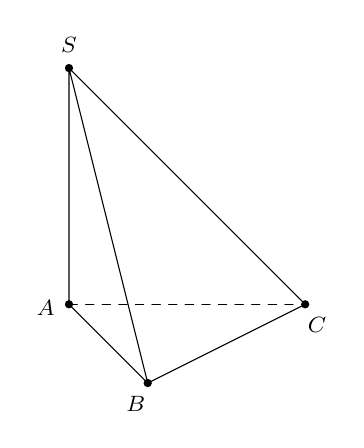
\begin{tikzpicture}[scale=1, font=\footnotesize, line join=round, line cap=round, >=stealth]
				\path 
				(0,0) coordinate (A)
				(1,-1) coordinate (B)
				(3,0) coordinate (C)
				(A)+(0,3) coordinate (S)
				;
				
				\draw (S)--(A)--(B)--(C)--cycle (S)--(B);
				\draw[dashed] (A)--(C);
				\foreach \p/\r in {A/190,B/-120,C/-60,S/90}
				\fill (\p) circle (1.5pt) node[shift={(\r:3mm)}]{$\p$};
			\end{tikzpicture}
		}
	}
\end{ex}
\begin{ex}%[Đề thi thử Sở Yên Bái - 22 - 23]%[Dự án 12EX-6-2023]%[Nhật Thiện]%[2D3B1-1]
	Cho $\displaystyle\int \dfrac{1}{x^2} \mathrm{\,d}x=F(x)+C$. Khẳng định nào sau đây đúng?
	\choice
	{$F'(x)=\ln x^2$}
	{\True $F'(x)=\dfrac{1}{x^2}$}
	{$F'(x)=-\dfrac{2}{x^3}$}
	{$F'(x)=-\dfrac{1}{x}$}
	\loigiai{
		Ta có $\displaystyle\int \dfrac{1}{x^2} \mathrm{\,d}x=F(x)+C$ suy ra $F'(x)=\dfrac{1}{x^2}$.
	}
\end{ex}
\begin{ex}%[Đề thi thử Sở Yên Bái - 22 - 23]%[Dự án 12EX-6-2023]%[Nhật Thiện]%[2D4B2-3]
	Cho số phức $z$ thỏa mãn $(2-i)z+3+16i=2(\bar{z}+i)$. Mô-đun của $z$ bằng
	\choice
	{\True $\sqrt{13}$}
	{$5$}
	{$13$}
	{$\sqrt{5}$}
\loigiai{
Đặt $z=a+bi$ ($a$, $b\in \mathbb{R}$).\\
Ta có
\begin{eqnarray*}
	& &(2-i)z+3+16i=2(\bar{z}+i)\\
	&\Leftrightarrow& (2-i)(a+bi)+3+16i=2(a-bi+i)\\
	&\Leftrightarrow& 2a+b-ai+2bi+3+16i=2a-2bi+2i\\
	&\Leftrightarrow& 2a+b+3 + (-a+2b+16)i=2a+(-2b+2)i\\
	&\Leftrightarrow& \heva{&2a+b+3=2a\\
	&-a+2b+16=-2b+2}\\
	&\Leftrightarrow& \heva{&b=-3\\&-a+4b=-14}\\
	&\Leftrightarrow& \heva{&a=2\\&b=-3.}
\end{eqnarray*}
Suy ra $z=2-3i$. Vậy $|z|=\sqrt{2^2+(-3)^2}=\sqrt{13}$.
}
\end{ex}
\begin{ex}%[Đề thi thử Sở Yên Bái - 22 - 23]%[Dự án 12EX-6-2023]%[Nhật Thiện]%[1D2B5-2]
	Một nhóm gồm $10$ học sinh trong đó có hai bạn $A$ và $B$ đứng ngẫu nhiên thành một hàng. Xác suất để hai bạn $A$ và $B$ đứng cạnh nhau là
	\choice
	{$\dfrac{2}{5}$}
	{$\dfrac{1}{4}$}
	{$\dfrac{1}{10}$}
	{\True $\dfrac{1}{5}$}
\loigiai{
Xét phép thử $T$: Xếp ngẫu nhiên $10$ học sinh thành một hàng.\\
Không gian mẫu của phép thử $T$ là $\Omega$ suy ra $n(\Omega)=10!$.\\
Gọi $A$ là biến cố ``hai bạn $A$ và $B$ đứng cạnh nhau''.\\
Hai bạn $A$, $B$ xếp cạnh nhau có $2!$ cách.\\
Xếp nhóm hai bạn $A$, $B$ và $8$ bạn còn lại có $9!$ cách.\\
Suy ra $n(A)=2!\cdot 9!$.\\
Vậy $\mathrm{P}(A)=\dfrac{n(A)}{n(\Omega)}=\dfrac{2!\cdot 9!}{10!}=\dfrac{1}{5}$.
}
\end{ex}

\begin{ex}%[Đề thi thử Sở Yên Bái - 22 - 23]%[Dự án 12EX-6-2023]%[Nhật Thiện]%[2D3B3-4]
	Tính thể tích $V$ của phần vật thể giới hạn bởi hai mặt phẳng $x=1$ và $x=3$, biết rằng khi cắt vật thể bởi mặt phẳng vuông góc với trục $Ox$ tại điểm có hoành độ $x$ ($1\le x\le 3$) thì được thiết diện là một hình chữ nhật có độ dài hai cạnh là $3x$ và $\sqrt{3x^2-2}$.
	\choice
	{$V=(32+2\sqrt{15})\pi$}
	{\True $V=\dfrac{124}{3}$}
	{$V=\dfrac{124\pi}{3}$}
	{$V=(32+2\sqrt{15})$}
\loigiai{
Diện tích thiết diện là $S(x)=3x\cdot \sqrt{3x^2-2}$.\\
Thể tích vật thể là
$$V=\displaystyle\int\limits_1^3 S(x) \mathrm{\,d}x=\displaystyle\int\limits_1^3 3x\sqrt{3x^2-2} \mathrm{\,d}x.$$
Đặt $t=\sqrt{3x^2-2}\Rightarrow t^2=3x^2-2\Rightarrow t \mathrm{\,d}t=3x \mathrm{\,d}x$.\\
Đổi cận $x=1\Rightarrow t=1$, $x=3\Rightarrow t=5$.\\
Khi đó, $V=\displaystyle\int\limits_1^5 t\cdot t \mathrm{\,d}t=\dfrac{t^3}{3}\Big|_1^5=\dfrac{5^3}{3}-\dfrac{1^3}{3}=\dfrac{124}{3}$.
}
\end{ex}

\begin{ex}%[Đề thi thử Sở Yên Bái - 22 - 23]%[Dự án 12EX-6-2023]%[Nhật Thiện]%[1H3K5-3]
	Cho hình chóp tứ giác đều $S.ABCD$ có cạnh đáy bằng $2a$, cạnh bên bằng $a\sqrt{5}$. Tính khoảng cách từ điểm $B$ đến mặt phẳng $(SCD)$.
	\choice
	{\True $a\sqrt{3}$}
	{$\dfrac{a\sqrt{5}}{2}$}
	{$\dfrac{a\sqrt{3}}{2}$}
	{$a$}
\loigiai{
\immini{Gọi $O$ là tâm hình vuông $ABCD$.\\
	Ta có $OB$ cắt $(SCD)$ tại $D$.\\
	Suy ra $\dfrac{\mathrm{d}(B,(SCD))}{\mathrm{d}(O,(SCD))}=\dfrac{BD}{OD}=2$.\\
	Hay $\mathrm{d}(B,(SCD))=2\mathrm{d}(O,(SCD))$.\\
	Gọi $M$ là trung điểm $CD$, do $\triangle OCD$ là tam giác cân nên $OM\perp CD$. \\
	Mà $SO\perp CD$ do $S.ABCD$ là hình chóp đều.\\
	Suy ra $CD\perp (SOM)$.}
{
\begin{tikzpicture}[scale=1, font=\footnotesize, line join=round, line cap=round, >=stealth]
	\path 
	(0,0) coordinate (A)
	(-2,-1) coordinate (B)
	(4,0) coordinate (D)
	($(B)+(D)-(A)$) coordinate (C)
	($(A)!.5!(C)$) coordinate (O)
	(O)+(0,4) coordinate (S)
	($(C)!.5!(D)$) coordinate (M)
	($(S)!.6!(M)$) coordinate (H)
	;
	\foreach \x/\y/\z in{S/O/M,O/M/C,O/H/M}
	\draw    pic[draw=black, angle eccentricity=2, angle radius=0.25cm]
	{right angle=\x--\y--\z}; %Góc vuông
	\draw (S)--(B)--(C)--(D)--cycle (S)--(C) (S)--(M);
	\draw[dashed] (S)--(A) (B)--(A)--(D) (A)--(C) (B)--(D) (O)--(S) (O)--(M) (O)--(H);
	\foreach \p/\r in {A/150,B/-120,C/-60,D/0,S/90,O/-90,M/-45,H/0}
	\fill (\p) circle (1.5pt) node[shift={(\r:3mm)}]{$\p$};
	
\end{tikzpicture}
}
\noindent Kẻ đường cao $OH$ trong tam giác $SOM$. \\
Ta có $OH\perp CD$ (do $CD\perp (SOM)$).\\
Mà $OH\perp SM$.\\
Suy ra $OH\perp (SCD)$ hay $OH=\mathrm{d}(O,(SCD))$.\\
Ta có $OD=\dfrac{1}{2}BD=\dfrac{AB\sqrt{2}}{2}=\dfrac{2a\sqrt{2}}{2}=a\sqrt{2}$.\\
Suy ra $SO=\sqrt{SD^2-OD^2}=\sqrt{\left(a\sqrt{5}\right)^2-\left(a\sqrt{2}\right)^2}=a\sqrt{3}$.\\
Xét tam giác vuông $SOM$, ta có
$$\dfrac{1}{OH^2}=\dfrac{1}{SO^2}+\dfrac{1}{OM^2}\Rightarrow OH=\dfrac{SO\cdot OM}{\sqrt{SO^2+OM^2}}=\dfrac{a\sqrt{3}\cdot a}{\sqrt{\left(a\sqrt{3}\right)^2+a^2}}=\dfrac{a\sqrt{3}}{2}.$$
Vậy $\mathrm{d}(B,(SCD))=2\mathrm{d}(O,(SCD))=2\cdot OH=2\cdot \dfrac{a\sqrt{3}}{2}=a\sqrt{3}$.
}
\end{ex}
\begin{ex}%[Đề thi thử Sở Yên Bái - 22 - 23]%[Dự án 12EX-6-2023]%[Nhật Thiện]%[2D1K2-6]
	Có bao nhiêu giá trị nguyên của tham số $m$ để hàm số $y=x^4-6x^2+mx$ có ba điểm cực trị?
	\choice
	{$17$}
	{\True $15$}
	{$3$}
	{$7$}
\loigiai{
Xét $y'=4x^3-12x+m$, cho $y'=0\Leftrightarrow 4x^3-12x+m=0\Leftrightarrow 4x^3-12x=-m$.\qquad $(1)$\\
Để hàm số $y=x^4-6x^2+mx$ có ba điểm cực trị thì phương trình $y'=0$ có ba nghiệm phân biệt.\\
Xét hàm số $y=g(x)=4x^3-12x$ trên $\mathbb{R}$, có $g'(x)=12x^2-12=0\Leftrightarrow \hoac{&x=1\\&x=-1.}$\\
Bảng xét dấu của hàm số $g(x)$ như sau
\begin{center}
	
\begin{tikzpicture}[scale=1, font=\footnotesize, line join=round, line cap=round, >=stealth]
\tkzTabInit[nocadre=false,lgt=1.2,espcl=2.5,deltacl=0.6]
{$x$ /0.6,$g'(x)$ /0.6,$g(x)$ /2}
{$-\infty$,$-1$,$1$,$+\infty$}
\tkzTabLine{,+,0,-,0,+,}
\tkzTabVar{-/$-\infty$,+/$8$,-/$-8$,+/$+\infty$}
\end{tikzpicture}
\end{center}
Dựa vào bảng biến thiên, để phương trình $(1)$ có $3$ nghiệm phân biệt khi và chỉ khi 
$$-8<-m<8\Leftrightarrow -8<m<8.$$
Mà $m\in \mathbb{Z}$ suy ra $m\in \{\pm 7;\pm 6;\pm 5;\pm 4;\pm 3;\pm 2;\pm 1;0\}$.\\
Vậy có $15$ giá trị nguyên của tham số $m$.
}
\end{ex}
\begin{ex}%[Đề thi thử Sở Yên Bái - 22 - 23]%[Dự án 12EX-6-2023]%[Nhật Thiện]%[2D3K1-1]
	Cho hàm số $y=f(x)$ xác định và có đạo hàm liên tục trên đoạn $[0;4]$ thỏa mãn $f(0)=1$ và $(2x+1)f'(x)-f(x)=(2x+1)\sqrt{2x+1}$. Tính $f(4)$.
	\choice
	{\True $15$}
	{$10$}
	{$27$}
	{$20$}
\loigiai{
Ta có
\begin{eqnarray*}
	& &(2x+1)f'(x)-f(x)=(2x+1)\sqrt{2x+1}\\
	&\Leftrightarrow & \dfrac{(2x+1)f'(x)-f(x)}{(2x+1)\sqrt{2x+1}}=1\\
	&\Leftrightarrow & \dfrac{f'(x)\cdot \sqrt{2x+1}-f(x)\cdot \dfrac{1}{\sqrt{2x+1}}}{2x+1}=1\\
	&\Leftrightarrow& \left[\dfrac{f(x)}{\sqrt{2x+1}}\right]'=1\\
	&\Leftrightarrow& \dfrac{f(x)}{\sqrt{2x+1}}=x+C.\qquad(*)
\end{eqnarray*}
Với $x=0$ thay vào $(*)$, ta được $\dfrac{f(0)}{\sqrt{2\cdot 0+1}}=0+C\Rightarrow C=1$.\\
Với $x=4$, $C=1$ thay vào $(*)$, ta được $\dfrac{f(4)}{\sqrt{2\cdot 4+1}}=4+1\Rightarrow f(4)=5\cdot 3=15$.
}
\end{ex}
\begin{ex}%[Đề thi thử Sở Yên Bái - 22 - 23]%[Dự án 12EX-6-2023]%[Nhật Thiện]%[2D2K6-2]
	Có bao nhiêu số nguyên $x$ thỏa mãn bất phương trình $\log_2\dfrac{x^2-3x+6}{243}<\log_3\dfrac{x^2-3x+6}{32}$?
	\choice
	{\True $176$}
	{$76$}
	{$189$}
	{$186$}
\loigiai{
Ta có
\begin{eqnarray*}
	& &\log_2 \dfrac{x^2-3x+6}{243}<\log_3 \dfrac{x^2-3x+6}{32}\\
	&\Leftrightarrow& \log_2 (x^2-3x+6)-\log_2 243<\log_3(x^2-3x+6)-\log_3 32\\
	&\Leftrightarrow& \log_2 3\cdot \log_3 (x^2-3x+6) -\log_3 (x^2-3x+6)<\log_2 3^5-\log_3 2^5\\
	&\Leftrightarrow& \log_3 (x^2-3x+6) \left[\log_2 3-1\right]<5\log_2 3-5\log_3 2\\
	&\Leftrightarrow& \log_3 (x^2-3x+6) \left[\log_2 3-1\right]<5\left[\log_2 3-\dfrac{1}{\log_2 3}\right]\\
	&\Leftrightarrow& \log_3 (x^2-3x+6) <5 \left[\dfrac{\log_23 +1}{\log_2 3}\right]\\
	&\Leftrightarrow& \log_3 (x^2-3x+6) < 5\log_3 6\\
	&\Leftrightarrow& \log_3 (x^2-3x+6) < \log_3 6^5\\
	&\Leftrightarrow& x^2-3x+6<6^5\\
	&\Leftrightarrow& x^2-3x-7770<0\\
	&\Leftrightarrow& \dfrac{3-\sqrt{31089}}{2}<x<\dfrac{3+\sqrt{31089}}{2}.
\end{eqnarray*}
Mà $x\in \mathbb{Z}$, suy ra có $176$ giá trị nguyên của $x$.
}
\end{ex}
\begin{ex}%[Đề thi thử Sở Yên Bái - 22 - 23]%[Dự án 12EX-6-2023]%[Nhật Thiện]%[2D1K3-1]
	Gọi $S$ là tập hợp tất cả các giá trị của tham số $m$ sao cho giá trị lớn nhất của hàm số $y=|x^3-3x+m|$ trên đoạn $[0;2]$ bằng $3$. Số phần tử của $S$ là
	\choice
	{$6$}
	{\True $2$}
	{$0$}
	{$1$}
\loigiai{
	Xét hàm số $g(x)=x^3-3x+m$.
	Ta có $g'(x)=0\Leftrightarrow 3x^2-3=0\Leftrightarrow \hoac{&x=1\\&x=-1.}$\\
	Bảng biến thiên của hàm $g(x)$ như sau
	\begin{center}
		
\begin{tikzpicture}[scale=1, font=\footnotesize, line join=round, line cap=round, >=stealth]
\tkzTabInit[nocadre=false,lgt=1.2,espcl=2.5,deltacl=0.6]
{$x$ /0.6,$g'(x)$ /0.6,$g(x)$ /2}
{$0$,$1$,$2$}
\tkzTabLine{,-,0,+,}
\tkzTabVar{+/$m$,-/$m-2$,+/$m+2$}
\end{tikzpicture}
	\end{center}
Dựa vào bảng biến thiên,
\begin{description}
	\item[Trường hợp 1.] $m+2< 0\Leftrightarrow m<- 2$.\\
	Khi đó $\max\limits_{x\in[0;2]} y=3\Leftrightarrow -(m-2)=3\Leftrightarrow m=-1$ (loại).
	\item[Trường hợp 2.] $\heva{&m<0\\&m+2>0}\Leftrightarrow \heva{&m<0\\&m>-2}\Leftrightarrow -2<m<0$.\\
	Khi đó $\max\limits_{x\in[0;2]} y=3\Leftrightarrow -(m-2)=3\Leftrightarrow m=-1$ (nhận).
	\item[Trường hợp 3.] $\heva{&m>0\\&m-2<0}\Leftrightarrow \heva{&m>0\\&m<2}\Leftrightarrow 0<m<2$.\\
	Khi đó $\max\limits_{x\in[0;2]} y=3\Leftrightarrow m+2=3\Leftrightarrow m=1$ (nhận).
	\item[Trường hợp 4.] $m-2>0\Leftrightarrow m>2$.\\
	Khi đó $\max\limits_{x\in[0;2]} y=3\Leftrightarrow m+2=3\Leftrightarrow m=1$ (loại).
\end{description}
Suy ra tập hợp $S=\{-1;1\}$, vậy $S$ có $2$ phần tử.
}
\end{ex}
\begin{ex}%[Đề thi thử Sở Yên Bái - 22 - 23]%[Dự án 12EX-6-2023]%[Nhật Thiện]%[2D1K1-3]
	Có bao nhiêu giá trị nguyên dương của tham số $m$ để hàm số $f(x)=\dfrac{1}{3}x^3-mx^2+(5m+6)x-1$ đồng biến trên $\mathbb{R}$?
	\choice
	{\True $6$}
	{$8$}
	{$5$}
	{$7$}
\loigiai{
Xét $f'(x)=x^2-2mx+(5m+6)$.\\
Hàm số đồng biến trên $\mathbb{R}$ khi và chỉ khi
$$\Delta'=(-m)^2-(5m+6)\le 0\Leftrightarrow -1\le m\le 6.$$
Mà $m$ là số nguyên dương suy ra có $6$ giá trị nguyên dương của tham số $m$ thỏa mãn.
}
\end{ex}
\begin{ex}%[Đề thi thử Sở Yên Bái - 22 - 23]%[Dự án 12EX-6-2023]%[Nhật Thiện]%[2D3K3-1]
	Bết $F(x)$ và $G(x)$ là hai nguyên hàm của hàm số $f(x)$ trên $\mathbb{R}$ và $\displaystyle\int\limits_0^4 f(x) \mathrm{\,d}x=F(4)-G(0)+2m$ ($m>0$). Gọi $S$ là diện tích hình phẳng giới hạn bởi các đường $y=F(x)$, $y=G(x)$, $x=0$ và $x=4$. Khi $S=8$ thì $m$ bằng
	\choice
	{$4$}
	{\True $1$}
	{$3$}
	{$2$}
\loigiai{
Ta có $\displaystyle\int\limits_0^4 f(x) \mathrm{\,d}x=F(4)-F(0)$ mà $\displaystyle\int\limits_0^4 f(x) \mathrm{\,d}x=F(4)-G(0)+2m$. \\
Suy ra $F(0)=G(0)-2m$ hay $F(0)-G(0)=-2m$.\\
Vì $F(x)$ và $G(x)$ là hai nguyên hàm của hàm số $f(x)$ trên $\mathbb{R}$ nên $$F(x)=G(x)+C\Rightarrow F(x)-G(x)=C=-2m.$$
Diện tích hình phẳng giới hạn bằng
\begin{eqnarray*}
	& &S=\displaystyle\int\limits_0^4 |F(x)-G(x)| \mathrm{\,d}x\Leftrightarrow 8=\displaystyle\int\limits_0^4 |-2m| \mathrm{\,d}x\\
	&\Leftrightarrow& 8=\displaystyle\int\limits_0^4 2m \mathrm{\,d}x\Leftrightarrow 8=2mx\big|_0^4 \Leftrightarrow 8=8m\\
	&\Leftrightarrow& m=1.
\end{eqnarray*}
}
\end{ex}
\begin{ex}%[Đề thi thử Sở Yên Bái - 22 - 23]%[Dự án 12EX-6-2023]%[Nhật Thiện]%[2D2K6-2]
	Số các giá trị nguyên của tham số $m$ để bất phương trình $\log_2(x^2+1)+1\ge \log_2(x^2+2mx+m+2)$ nghiệm đúng với $\forall x\in \mathbb{R}$ là
	\choice
	{$3$}
	{$1$}
	{$0$}
	{\True $2$}
\loigiai{
	Điều kiện $x^2+2mx+m+2>0$, $\forall x\in\mathbb{R}$.\\
	$\Leftrightarrow \Delta'=m^2-4(m+2)<0\Leftrightarrow m^2-4m-8<0\Leftrightarrow 2-2\sqrt{3}<m<2+2\sqrt{3}$.\\
Ta có
\begin{eqnarray*}
	& &\log_2(x^2+1)+1\ge \log_2(x^2+2mx+m+2)\\
	&\Leftrightarrow & \log_2\left[2(x^2+1)\right]\ge \log_2 (x^2+2mx+m+2)\\
	&\Leftrightarrow & 2(x^2+1)\ge x^2+2mx+m+2\\
	&\Leftrightarrow & x^2-2mx-m\ge 0,\ \forall x\in \mathbb{R}.
\end{eqnarray*}
Bất phương trình có nghiệm đúng với mọi $x\in \mathbb{R}$ khi và chỉ khi 
\begin{eqnarray*}
	& &x^2-2mx-m\ge 0, \forall x\in \mathbb{R}\\
	&\Leftrightarrow& \Delta'=m^2+4m\le 0\\
	&\Leftrightarrow& -4\le m\le 0.
\end{eqnarray*}
Mà $m\in \mathbb{Z}$, so sánh với điều kiện, vậy có $2$ giá trị của tham số $m$ thỏa mãn.
}
\end{ex}
\begin{ex}%[Đề thi thử Sở Yên Bái - 22 - 23]%[Dự án 12EX-6-2023]%[Nhật Thiện]%[2H3K3-2]
	Trong không gian $Oxyz$, cho mặt phẳng $(P)\colon 2x+2y-z-3=0$, đường thẳng $d\colon \dfrac{x+1}{1}=\dfrac{y-1}{1}=\dfrac{z}{2}$ và điểm $A(2;2;-1)$. Phương trình đường thẳng $\Delta$ qua $A$ cắt $d$ và song song với $(P)$ là
	\choice
	{$\dfrac{x-2}{3}=\dfrac{y-2}{-3}=\dfrac{z+1}{-2}$}
	{\True $\dfrac{x-2}{3}=\dfrac{y-2}{7}=\dfrac{z+1}{20}$}
	{$\dfrac{x+2}{2}=\dfrac{y+2}{-3}=\dfrac{z-1}{-2}$}
	{$\dfrac{x+2}{3}=\dfrac{y+2}{7}=\dfrac{z-1}{20}$}
\loigiai{
Giả sử $\Delta$ cắt $d$ tại $B$, suy ra $B(t-1;t+1;2t)$.\\
Khi đó $\Delta$ qua $A$ và $B$ nên nhận $\vec{AB}=(t-3;t-1;2t+1)$ làm một véc-tơ chỉ phương.\\
Mà $\Delta$ song song với $(P)$ nên $\vec{AB}\perp \vec{n}$ với $\vec{n}=(2;2;-1)$ là một véc-tơ pháp tuyến của $(P)$.\\
Ta có $\vec{AB}\perp \vec{n}\Leftrightarrow \vec{AB}\cdot \vec{n}=0\Leftrightarrow 2(t-3)+2(t-1)-1(2t+1)=0\Leftrightarrow 2t-9=0\Leftrightarrow t=\dfrac{9}{2}$.\\
Đường thẳng $\Delta$ qua $A(2;2;-1)$ và nhận $\vec{AB}=\left(\dfrac{3}{2};\dfrac{7}{2};10\right)=\dfrac{1}{2}\left(3;7;20\right)$ làm một véc-tơ chỉ phương.\\
Phương trình đường thẳng $\Delta$ là $$\dfrac{x-2}{3}=\dfrac{y-2}{7}=\dfrac{z+1}{20}.$$
}
\end{ex}
\begin{ex}%[Đề thi thử Sở Yên Bái - 22 - 23]%[Dự án 12EX-6-2023]%[Nhật Thiện]%[2D4K4-2]
	Trên tập số phức, xét phương trình $z^2-2(2m-1)z+m^2=0$ ($m$ là số thực). Có bao nhiêu giá trị của $m$ để phương trình đó có hai nghiệm phân biệt $z_1$, $z_2$ thỏa mãn $|z_1|^2+|z_2|^2=2$?
	\choice
	{$4$}
	{$3$}
	{\True $2$}
	{$1$}
\loigiai{
Xét $\Delta'=(2m-1)^2-m^2=3m^2-4m+1$.
\begin{description}
	\item[Trường hợp 1.] $\Delta'\ge 0\Leftrightarrow 3m^2-4m+1\ge0\Leftrightarrow m\le\dfrac{1}{3}$ hoặc $m\ge1$.\\
	Khi đó phương trình đã cho có hai nghiệm thực $z_1$, $z_2$.\\
	Vì $a\cdot c=m^2\ge 0$ nên phương trình có hai nghiệm $z_1\cdot z_2\ge 0$ hoặc $z_1\cdot z_2\le 0$.\\
	Suy ra 
	\begin{eqnarray*}
		& &z_1^2+z_2^2=2\Leftrightarrow z_1^2+z_2^2+2z_1 z_2=2+2z_1 z_2\\
		&\Leftrightarrow& \left(z_1+z_2\right)^2=2+2z_1z_2\\
		&\Leftrightarrow& \left[2(2m-1)\right]^2=2+2m^2\\
		&\Leftrightarrow& 4(4m^2-4m+1)=2+2m^2\\
		&\Leftrightarrow& 14m^2-16m+2=0\\
		&\Leftrightarrow& \hoac{&m=1\text{ (nhận)}\\&m=\dfrac{1}{7}.\text{ (nhận)}}
	\end{eqnarray*}
	\item[Trường hợp 2.] $\Delta'<0\Leftrightarrow \dfrac{1}{3}<m<1$.\\
	Khi đó phương trình đã cho có hai nghiệm phức $z_1$, $z_2$.\\
	Suy ra 
	\begin{eqnarray*}
		& &|z_1|^2+|z_2|^2=2\Leftrightarrow 2|z_1|^2=2\Leftrightarrow |z_1|^2=1\\
		&\Leftrightarrow& z_1\overline{z_1}=1\Leftrightarrow z_1z_2=1\Leftrightarrow m^2=1\\
		&\Leftrightarrow& \hoac{&m=1&\text{ (loại)}\\&m=-1.&\text{ (loại)}}
	\end{eqnarray*}
\end{description}
Vậy có $2$ giá trị của tham số $m$ thỏa mãn.
}
\end{ex}
\begin{ex}%[Đề thi thử Sở Yên Bái - 22 - 23]%[Dự án 12EX-6-2023]%[Nhật Thiện]%[2D4K5-1]
	Xét số phức $z=a+bi$ ($a$, $b\in \mathbb{R}$) thỏa mãn $|z-4-3i|=\sqrt{5}$. Tính giá trị của biểu thức $P=a+b$ khi $|z+1-3i|+|z-1+i|$ đạt giá trị lớn nhất?
	\choice
	{$P=4$}
	{$P=6$}
	{\True $P=10$}
	{$P=8$}
\loigiai{
\immini{Giả sử số phức $z=a+bi$ có điểm biểu diễn $M(a;b)$.\\
	Suy ra tập hợp điểm $M$ là đường tròn $$(C)\colon (x-4)^2+(y-3)^2=5$$ có tâm $I(4;3)$ và bán kính $R=\sqrt{5}$.\\
	Gọi $A(-1;3)$ và $B(1;-1)$ lần lượt là hai điểm biểu diễn cho số phức $z_1=-1+3i$ và $z_2=1-i$.
	}
{
	\begin{tikzpicture}[scale=1, font=\footnotesize, line join=round, line cap=round, >=stealth]
		\begin{scope}[scale=.8]
			\def\r{sqrt(5)}
			\path 
			(4,3) coordinate (I)
			(-1,3) coordinate (A)
			(1,-1) coordinate (B)
			(6,4) coordinate (M)
			($(A)!.5!(B)$) coordinate (E)
			;
			\draw[name path=dt1] (I) circle (\r);
			\path[name path=am] (A)--(M);
%			\path[name intersections={of=am and dt1}] (intersection-2) coordinate (M');
			\draw ($(M)!1.2!(E)$)--($(E)!1.2!(M)$);
			\draw (A)--(B)--(M)--cycle;
%			\draw (E)--(M');
			\foreach \p/\r in {A/90,B/-120,M/-20,E/150,I/135}
			\fill (\p) circle (1.5pt) node[shift={(\r:3mm)}]{$\p$};
		\end{scope}
	\end{tikzpicture}
}
\noindent Ta có 
\begin{eqnarray*}
	& &Q=|z+1-3i|+|z-1+i|=MA+MB \le \sqrt{2(MA^2+MB^2)}\\
	&\Leftrightarrow& Q^2\le 2(MA^2+MB)^2.
\end{eqnarray*}
Gọi $E(0;1)$ là trung điểm $AB$ nên $ME^2=\dfrac{MA^2+MB^2}{2}-\dfrac{AB^2}{4}$.\\
Do đó $Q^2\le 2(MA^2+MB^2)=4ME^2+AB^2$ mà $ME\le EI+R=3\sqrt{5}$ suy ra
\begin{eqnarray*}
	& &Q^2\le 4\cdot \left(3\sqrt{5}\right)^2+\left(2\sqrt{5}\right)^2=200\\
	&\Rightarrow& Q\le 10\sqrt{2}.
\end{eqnarray*}
Dấu bằng xảy ra khi $MA=MB$ hay $M$ là giao điểm của đường thẳng $EI\colon x-2y+2=0$ với đường tròn $(C)$.\\
Tọa độ $M$ thỏa hệ
$$\heva{&x-2y+2=0\\&(x-4)^2+(y-3)^2=5}\Leftrightarrow \heva{&x=2y-2\\&(2y-2-4)^2+(y-3)^2=5}\Leftrightarrow \heva{&x=2y-2\\&\hoac{&y=2\\&y=4}}\Leftrightarrow \hoac{&\heva{&x=2\\&y=2}\\&\heva{&x=6\\&y=4.}}$$
Với $M(2;2)$ suy ra $Q=MA+MB=2\sqrt{10}$.\\
Với $M(6;4)$ suy ra $Q=MA+MB=10\sqrt{2}$.\\
Suy ra $M(6;4)$ thỏa mãn bài toán. Vậy $P=a+b=6+4=10$.
}
\end{ex}
\begin{ex}%[Đề thi thử Sở Yên Bái - 22 - 23]%[Dự án 12EX-6-2023]%[Nhật Thiện]%[2H1K3-2]
	Cho hình chóp $S.ABC$ có đáy là tam giác vuông tại $A$ và $AB=\sqrt{3}$, $AC=\sqrt{7}$, $SA=1$. Hai mặt bên $(SAB)$ và $(SAC)$ lần lượt tạo với mặt đáy các góc bằng $45^\circ$ và $60^\circ$. Thể tích của khối chóp đã cho bằng.
	\choice
	{\True $\dfrac{1}{2}$}
	{$\dfrac{7}{6}$}
	{$\dfrac{\sqrt{3}}{2}$}
	{$\dfrac{7\sqrt{7}}{6}$}
\loigiai{
\immini{Gọi $H$ là hình chiếu vuông góc của $S$ lên $(ABC)$.\\
Kẻ $HM$, $HN$ lần lượt vuông góc với $AB$, $AC$ tại $M$ và $N$.\\
Khi đó $\heva{&SH\perp AB\\&HM\perp AB}\Rightarrow AB\perp SM$, tương tự $AC\perp SN$.\\
Ta có $\heva{&(SAB)\cap (ABC)=AB\\&SM\subset (SAB),\ SM\perp AB\\&HM\subset (ABC),\ HM\perp AB.}$\\
Suy ra góc giữa $(SAB)$ và $(ABC)$ là góc $\widehat{SMH}$ và $\widehat{SMH}=45^\circ$.\\
Tương tự, góc giữa $(SAC)$ và $(ABC)$ là góc $\widehat{SNH}$ và $\widehat{SNH}=60^\circ$.}{
	\begin{tikzpicture}[scale=1, font=\footnotesize, line join=round, line cap=round, >=stealth]
		\path 
		(0,0) coordinate (B)
		(1,-1.5) coordinate (A)
		(4,0) coordinate (C)
		($(B)!.6!(C)$) coordinate (x)
		($(A)!.7!(x)$) coordinate (H)
		(H)+(0,4) coordinate (S)
		($(H)+(C)-(A)$) coordinate (m1)
		(intersection of H--m1 and A--B) coordinate (M)
		($(H)+(B)-(A)$) coordinate (m2)
		(intersection of H--m2 and A--C) coordinate (N)
		;
		\foreach \x/\y/\z in{H/M/B,H/N/C,S/H/M,B/A/C}
		\draw    pic[draw=black, angle eccentricity=2, angle radius=0.25cm]
		{right angle=\x--\y--\z}; %Góc vuông
		\draw (S)--(B)--(A)--(C)--cycle (S)--(A) (S)--(M) (S)--(N);
		\draw[dashed] (B)--(C) (H)--(M) (H)--(N) (S)--(H);
		\foreach \p/\r in {A/190,B/-120,C/-60,S/90,H/-90,M/-135,N/-45}
		\fill (\p) circle (1.5pt) node[shift={(\r:3mm)}]{$\p$};
	\end{tikzpicture}
}
\noindent Ta có
$\heva{&HM\cdot \tan 45^\circ=HS\\&HN\cdot \tan 60^\circ=HS}\Leftrightarrow \heva{&HM=HS\\&HN\sqrt{3}=HS.}$\\
Mà $SH^2=SA^2-AH^2=SA^2-HM^2-HN^2=1-SH^2-\dfrac{SH^2}{3}$.\\
$\Leftrightarrow SH^2=\dfrac{3}{7}\Rightarrow SH=\dfrac{\sqrt{21}}{7}$.\\
Thể tích của khối chóp bằng
$$V=\dfrac{1}{3}\cdot S_{ABC}\cdot SH=\dfrac{1}{3}\cdot \dfrac{1}{2}\cdot AB\cdot AC\cdot SH=\dfrac{1}{6}\cdot \sqrt{3}\cdot \sqrt{7}\cdot \dfrac{\sqrt{21}}{7}=\dfrac{1}{2}.$$
}
\end{ex}
\begin{ex}%[Đề thi thử Sở Yên Bái - 22 - 23]%[Dự án 12EX-6-2023]%[Nhật Thiện]%[2D1K1-3]
	Có bao nhiêu giá trị nguyên của tham số $m$ trong đoạn $[-10;10]$ để hàm số $y=\left|\dfrac{mx+3}{x+m+2}\right|$ đồng biến trên khoảng $(1;+\infty)$?
	\choice
	{\True $9$}
	{$0$}
	{$10$}
	{$8$}
\loigiai{
Xét hàm số $g(x)=\dfrac{mx+3}{x+m+2}$.\\
Hàm số $y=\left|\dfrac{mx+3}{x+m+2}\right|=|g(x)|$ đồng biến trên khoảng $(1;+\infty)$.
\begin{description}
	\item[Trường hợp 1.] 
	\begin{eqnarray*}
		& &\heva{&g(1)\ge 0\\&g'(x)>0,\ \forall x\in (1;+\infty)}\Leftrightarrow \heva{&\dfrac{m+3}{m+3}=1\ge 0\text{ (luôn đúng)}\\&m^2+2m-3>0\\&-m-2\le 1}\Leftrightarrow \heva{&m<-3\text{ hoặc }m>1\\&m\ge -3}\\
		&\Leftrightarrow& m>1.
	\end{eqnarray*}
	\item[Trường hợp 2.]
	$$\heva{&g(1)\le 0\\&g'(x)<0,\ \forall x\in (1;+\infty)}\Leftrightarrow \heva{&\dfrac{m+3}{m+3}=1\le 0\text{ (vô lý)}\\&m^2+2m-3<0\\&-m-2\le 1.}$$
	Trường hợp này loại.
\end{description}
Mà $m$ là số nguyên và $m\in [-10;10]$, suy ra $1<m\le 10$.\\
Vậy có $9$ giá trị của tham số $m$.
}
\end{ex}
\begin{ex}%[Đề thi thử Sở Yên Bái - 22 - 23]%[Dự án 12EX-6-2023]%[Nhật Thiện]%[2H3G3-8]
	Trong không gian $Oxyz$, cho điểm $A(1;2;-3)$ và mặt phẳng $(P)\colon 2x+2y-z+9=0$. Đường thẳng $d$ đi qua $A$ và vuông góc với mặt phẳng $(Q)\colon 3x+4y-4z+5=0$ cắt mặt phẳng $(P)$ tại điểm $B$. Điểm $M$ nằm trong mặt phẳng $(P)$, nhìn đoạn $AB$ dưới góc vuông và độ dài $MB$ lớn nhất. Tính độ dài $MB$.
	\choice
	{$MB=\dfrac{\sqrt{41}}{2}$}
	{$MB=\dfrac{\sqrt{5}}{2}$}
	{\True $MB=\sqrt{5}$}
	{$MB=\sqrt{41}$}
	\loigiai{
	\immini{
		Đường thẳng $d$ đi qua $A(1;2;-3)$ và vuông góc với $(Q)$ có dạng $\heva{& x=1+3t\\& y=2+4t\\& z=-3-4t.}$\\
		Ta có $\heva{& B(1+3t; 2+4t; -3-4t)\in d\\& B\in (P)\colon 2x+2y-z+9=0.}$
	}{
		\begin{tikzpicture}[scale=0.8, font=\footnotesize, line join=round, line cap=round, >=stealth]
			\tkzDefPoints{0/0/E,-1.5/-1.5/F,4/-1.5/G,1/2/A,1/-0.5/M,2.5/-1/B}
			\path
			(0,0) coordinate (E)
			(-1.5,-1.5) coordinate (F)
			(4,-1.5) coordinate (G)
			(1,2) coordinate (A)
			(1,-.5) coordinate (M)
			(2.5,-1) coordinate (B)
			;
			\coordinate (H) at ($(E)+(G)-(F)$);
			\path
			(intersection of A--M and E--H) coordinate (I)
			(intersection of A--B and E--H) coordinate (J)
			(intersection of A--B and F--G) coordinate (K)
			;
			
			\coordinate (d) at ($(A)!3/2!(B)$);
			\tkzDrawLines[add=0.5cm and 0cm](A,B)
			\draw (I)--(E)--(F)--(G)--(H)--(J) (A)--(M)--(B) (K)--(d);
			\draw[dashed] (I)--(J) (B)--(K);
			\foreach \p/\r in {A/0,B/0,M/180}
			\fill (\p) circle (1.5pt) node[shift={(\r:3mm)}]{$\p$};
			\foreach \x/\y/\z in{G/F/E,B/M/A}
			\draw    pic[draw=black, angle eccentricity=2, angle radius=0.25cm]
			{right angle=\x--\y--\z}; %Góc vuông
		\end{tikzpicture}
	}
	\noindent
	Suy ra
	
	\begin{eqnarray*}
		& & 2(1+3t)+2(2+4t)-(-3-4t)+9=0\\
		&\Leftrightarrow & 18t+18=0 \Leftrightarrow t=-1.
	\end{eqnarray*}
	Do đó $B(-2; -2; 1) \Rightarrow AB=\sqrt{9+16+16}=\sqrt{41}$.\\
	Xét $\triangle MAB$ vuông tại $M$ có $MB^2=AB^2-MA^2=41-MA^2$.\\
	Khi đó $MB$ lớn nhất khi $MA$ nhỏ nhất $\Leftrightarrow$ $M$ là hình chiếu của $A$ trên $(P)$ (do $M\in (P)$).\\
	Nên $MA_{\min}=\mathrm{d}(A,(P))=\dfrac{\left|2+4+3+9\right|}{\sqrt{2^2+2^2+(-1)^2}}=6$.\\
	Vậy $MB_{\max}=\sqrt{41-MA^2}=\sqrt{5}$.
}
\end{ex}
\begin{ex}%[Đề thi thử Sở Yên Bái - 22 - 23]%[Dự án 12EX-6-2023]%[Nhật Thiện]%[2D2G5-5]
	Tất cả các cặp số nguyên $(x;y)$ thỏa mãn điều kiện $\log_2(x+2y)+x^2+2y^2+3xy-x-y=0$ với $x+y>0$, $-20\le x\le 20$ là
	\choice
	{$41$}
	{\True $10$}
	{$6$}
	{$19$}
\loigiai{
Điều kiện $x+y>0$, ta có
\begin{eqnarray*}
	& &\log_2(x+2y)+x^2+2y^2+3xy-x-y=0\\
	&\Leftrightarrow& \log_2 \dfrac{(x+y)(x+2y)}{x+y}+x^2+2y^2+3xy-x-y=0\\
	&\Leftrightarrow& \log_2 \left[(x+y)(x+2y)\right]-\log_2(x+y)+x^2+2y^2+3xy-x-y=0\\
	&\Leftrightarrow& \log_2 (x^2+2y^2+3xy)+x^2+y^2+3xy=\log_2(x+y)+x+y.\qquad(1)
\end{eqnarray*}
Xét hàm số $f(t)=\log_2t+t$ trên $(0;+\infty)$. \\
Ta có $f'(t)=\dfrac{1}{t}+1>0$, $\forall t\in (0;+\infty)$ nên hàm số $f(t)$ đồng biến trên $(0;+\infty)$.\\
Do đó
\begin{eqnarray*}
	(1)&\Leftrightarrow& f(x^2+2y^2+3xy)=f(x+y)\Leftrightarrow x^2+2y^2+3xy=x+y\\
	&\Leftrightarrow& (x+y)(x+2y)=x+y\Leftrightarrow (x+y)(x+2y-1)=0
\end{eqnarray*}
Vì $x+y>0$ nên $x+2y-1=0\Leftrightarrow x=1-2y$.\\
Do $x\in [-20;20]$ suy ra $-20\le 1-2y\le 20\Leftrightarrow -21\le -2y\le 19\Leftrightarrow -\dfrac{19}{2}\le y\le \dfrac{21}{2}$.\\
Từ điều kiện $x+y>0$ và $x=1-2y$, ta có $x+y=1-y>0\Leftrightarrow y<1$.\\
Mà $y\in \mathbb{Z}$ nên $y\in \{-9,-8,\ldots,0\}$.\\
Với mỗi giá trị của $y$ tương ứng có $1$ giá trị của $x$.\\
Vậy có $10$ cặp số nguyên $(x;y)$ thỏa mãn.
}
\end{ex}
\Closesolutionfile{ans}
\indapan{10}{ans/ans-2-TT-20-SoGDDT-YenBai-23}


